%----------------------------------------------------------------------------
\chapter{Evaluation} \label{evaluation}
%----------------------------------------------------------------------------

This chapter collects and evaluates the results of the measurements that apply enhancements ot the application. 

%%----------------------------------------------------------------------------
%\section{Continuous Delivery}
%%----------------------------------------------------------------------------

%----------------------------------------------------------------------------
\section{Kafka}
%----------------------------------------------------------------------------

The results of measurements where the Kafka enhancement is applied can be seen in Figure \ref{fig:kafka-results-pod-failure} and Figure \ref{fig:kafka-results-pod-kill}. The diagrams show that using Kafka did not improve the dependability of the application, in fact, in case of the "\texttt{pod-failure}" fault profile, it produced worse results.

The reason for these results hides in integrating the Kafka cluster into the system with default configurations. Although Kafka is widely popular for its fault tolerance, it cannot guarantee the advertised level of robustness with the basic setup. Some of the causes are described below.

\paragraph{Memory based message logs -}Kafka keeps track of the messages in each topic that were already processed by consumer groups and also that are still waiting to be handled. Consumers use this data, to know which messages should they query from the brokers. By default these so called "commit logs" are not persisted and only stored in-memory. This leads to the fact, that when the Kafka brokers encounter an error and are restarted, the commit logs can be lost and the consumers do not know where to continue the message processing, which in turn can lead to data loss.

\paragraph{Minimum number of nodes -}Both Kafka and Zookeeper clusters need at least three nodes in order to be able to support various kinds of distributed algorithms (\eg leader election in case of Kafka topic partitioning). But when the number of nodes drop below this minimum number -- for example during fault injection --, Kafka may drop producer and consumer requests because the brokers responsible for a topic may be unavailable.

Despite the results, Kafka could replace the original messaging subsystem, however only with proper configurations and additional tools supporting the fault tolerance of Kafka, but this topic exceeds the scope of the thesis project.

\begin{figure}[h]
	\centering
	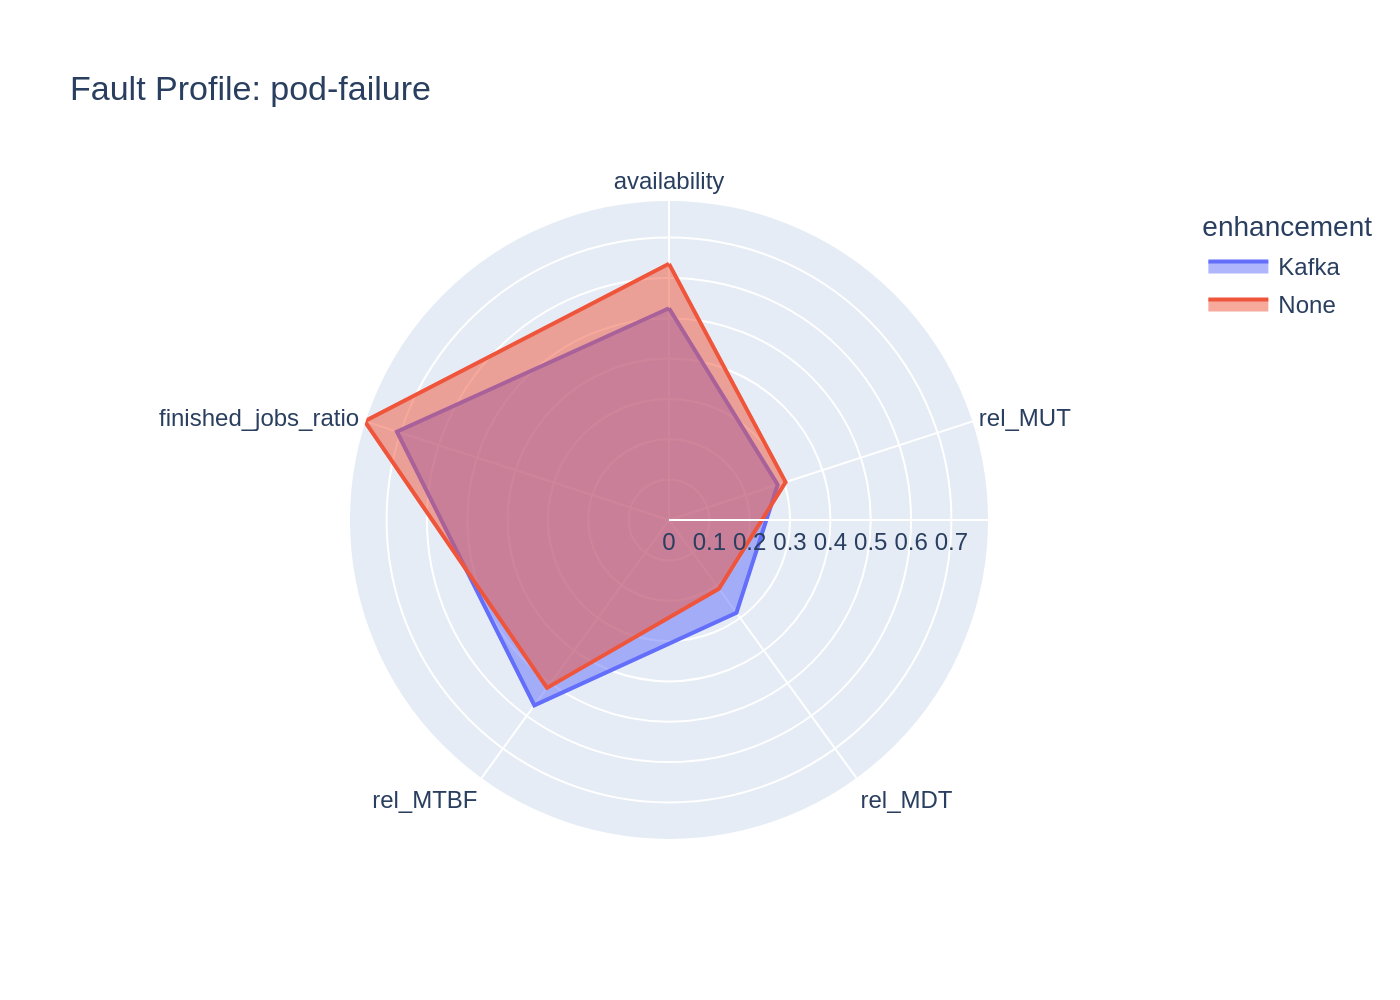
\includegraphics[width=140mm, keepaspectratio]{figures/kafka_with_base_pod-failure.png}
	\caption{Kafka enhancement - pod-failure fault profile}
	\label{fig:kafka-results-pod-failure}
\end{figure}

%\begin{itemize}
%	\item turns out, adding the complexity of kafka integration does not improve dependability metrics -- at least with the basic configurations (just Kafka and Zookeeper nodes 3-3 / 5-5), Kafka needs further components, hardening for robust operation -- log persistence (memory lost on pod-failure)
%\end{itemize}

\begin{figure}[h]
	\centering
	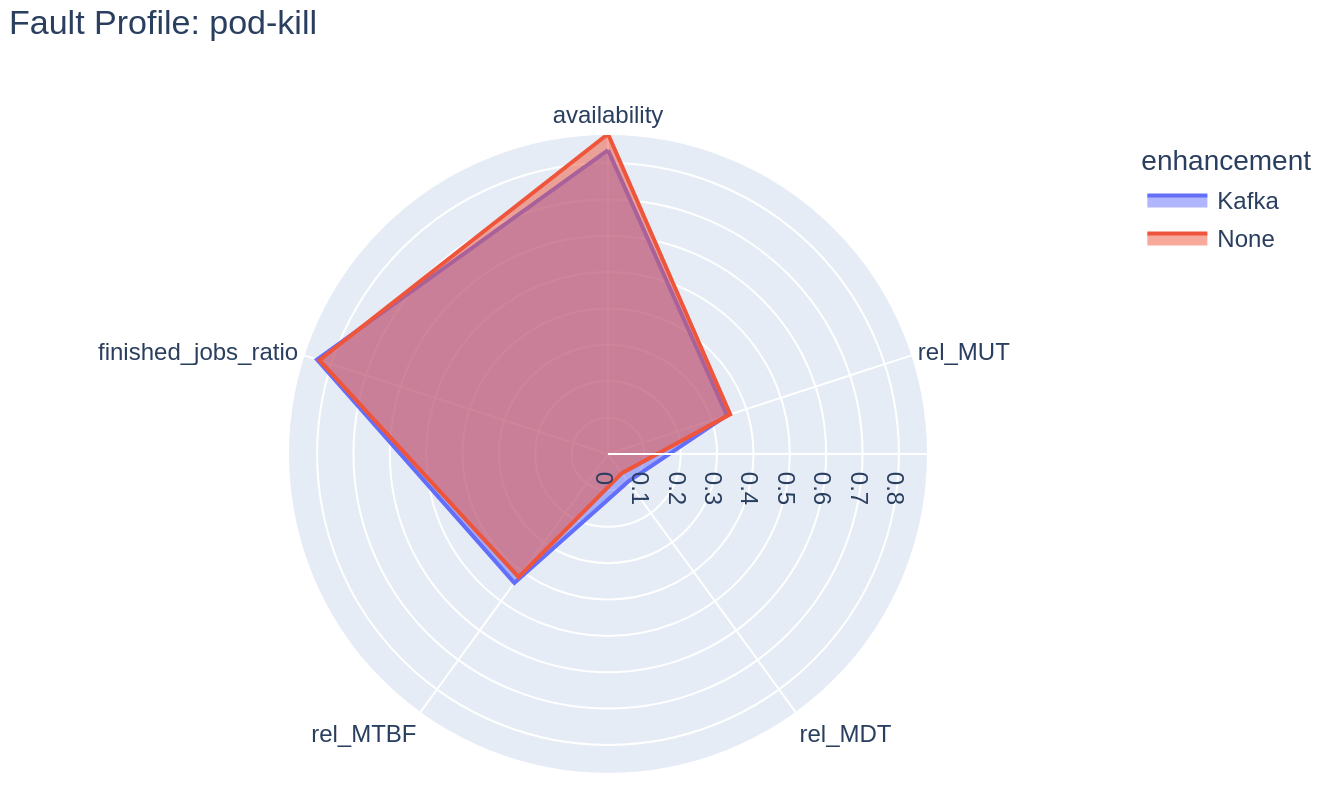
\includegraphics[width=140mm, keepaspectratio]{figures/kafka_with_base_pod-kill.png}
	\caption{Kafka enhancement - pod-kill fault profile}
	\label{fig:kafka-results-pod-kill}
\end{figure}

%\begin{itemize}
%	\item pod-kill scenario approximately is the same with Kafka (as described before, pod-kill is less severe than pod-failure chaos)
%\end{itemize}

%----------------------------------------------------------------------------
\section{Heartbeats}
%----------------------------------------------------------------------------

The results of measurements where the Heartbeats enhancement is applied can be seen in Figure \ref{fig:heartbeats-results-pod-failure} and Figure \ref{fig:heartbeats-results-pod-kill}. The diagrams show that this simple algorithm could improve the dependability of the application.

In case of "\texttt{pod-failure}" fault profile, the enhancement caused significant increase in \texttt{finished\_jobs\_ratio}, introduced a lower frequency of faults (increased \texttt{rel\_MTBF}), while the \texttt{availability} approximately stayed the same compared to the baseline results.

The "\texttt{pod-kill}" fault profile was handled considerably better with Heartbeats, than without it. All metrics improved greatly by the enhancement.

These outcomes prove that sometimes it is well worth to check the applications itself for possible improvements before jumping into integrating complex third party tools. However, one have to keep in mind, that Heartbeats only covered one failure scenario -- the unexpected stops of worker components --, so the system is still vulnerable to backend or database outages. Another thing to notice, that this solution depends more on reliable messaging than the original implementation. This means that, if the messaging subsystem is corrupted, Heartbeats may have no effect on the dependability metrics.


%\begin{itemize}
%	\item the simple algorithm could improve the jobs ratio in both cases
%	\item pod-kill was considerably better
%	\item heartbeat is weak against backend of db downtime - but there are more worker components in average, so they are more likely to fail statistically -- improve: backend and db in HA
%\end{itemize}

\begin{figure}[h]
	\centering
	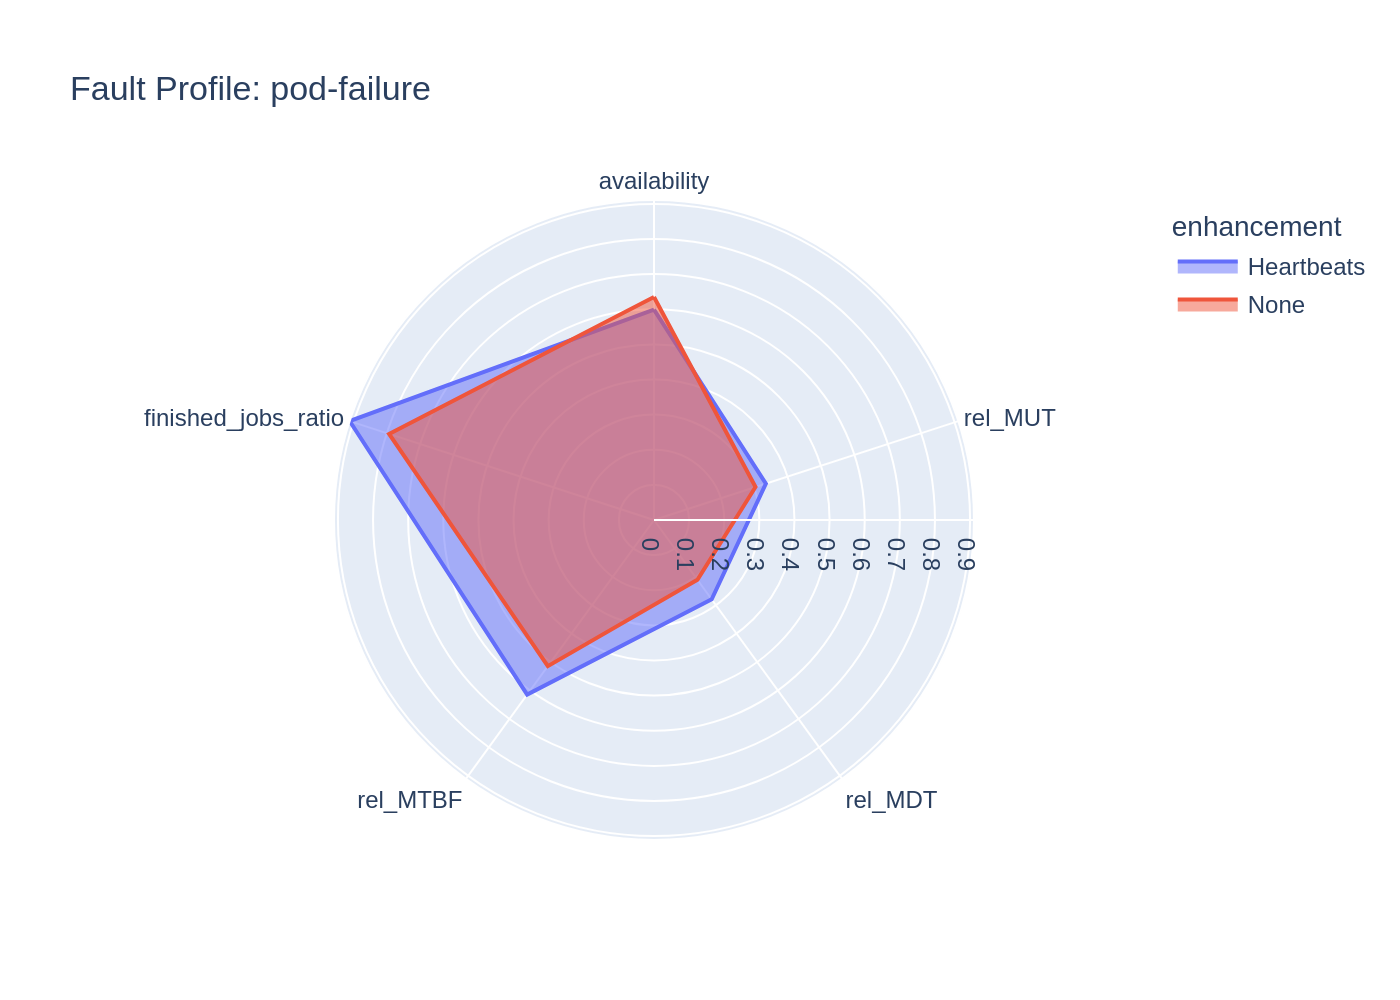
\includegraphics[width=140mm, keepaspectratio]{figures/heartbeats_with_base_pod-failure.png}
	\caption{Heartbeats enhancement - pod-failure fault profile}
	\label{fig:heartbeats-results-pod-failure}
\end{figure}

\begin{figure}[h]
	\centering
	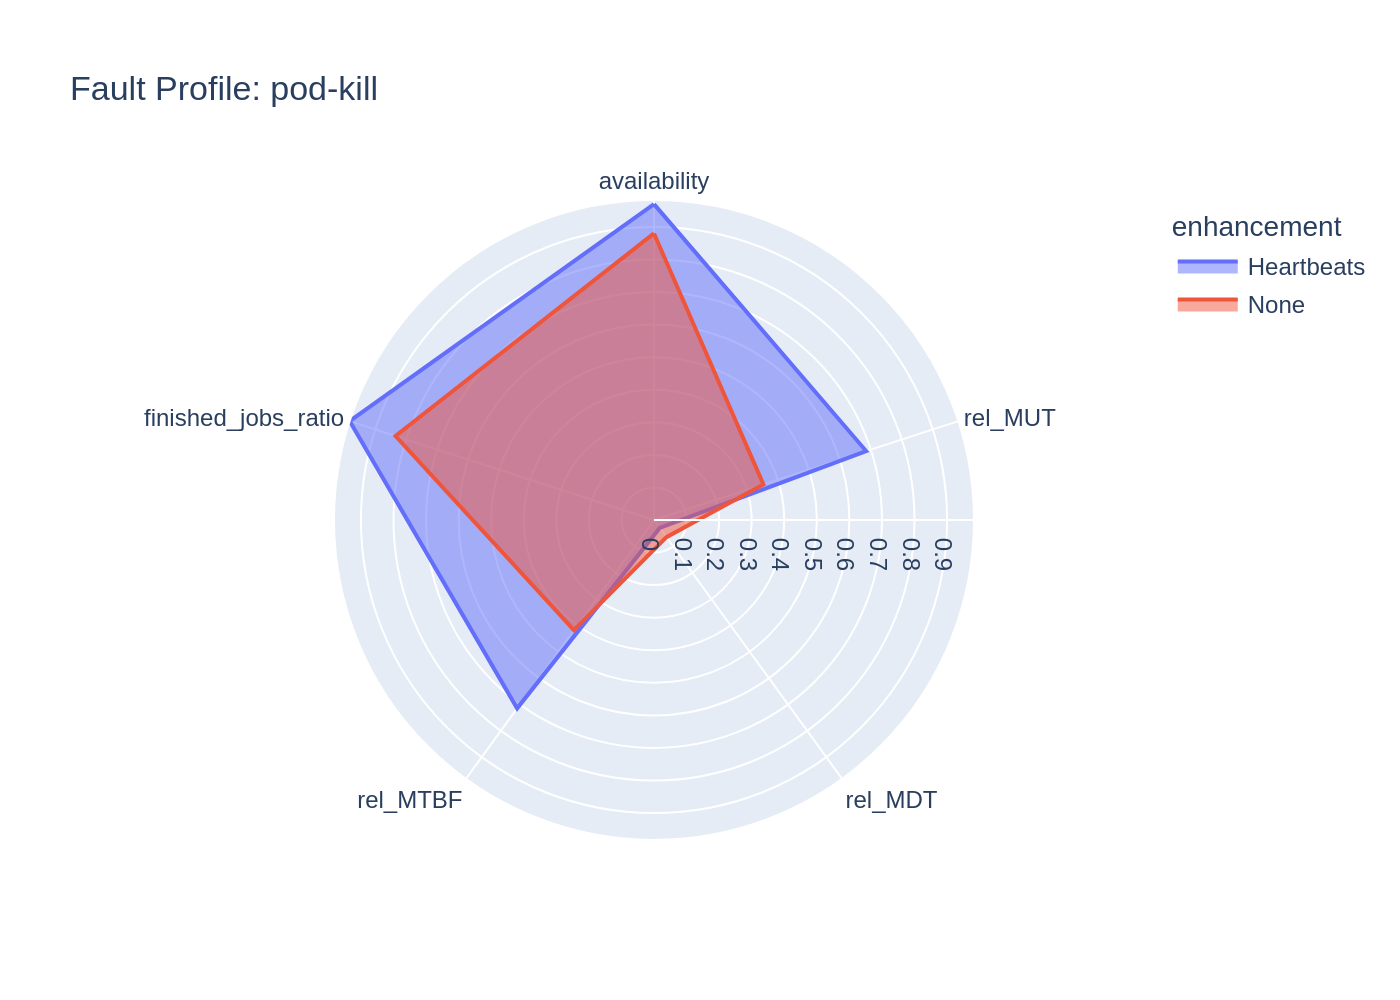
\includegraphics[width=140mm, keepaspectratio]{figures/heartbeats_with_base_pod-kill.png}
	\caption{Heartbeats enhancement - pod-kill fault profile}
	\label{fig:heartbeats-results-pod-kill}
\end{figure}

%----------------------------------------------------------------------------
\section{Combined Enhancements}
%----------------------------------------------------------------------------

The results of measurements where both Kafka and the Heartbeats enhancements are applied can be seen in Figure \ref{fig:combined-results-pod-failure} and Figure \ref{fig:combined-results-pod-kill}.

Apart from increasing the \texttt{availability} during the "\texttt{pod-kill}" fault injection, combining the two enhancements did not improve the dependability of the system. The reason for that is related to the weaknesses of the Kafka deployment in the current configuration described above. Because in this combined scenario the messaging system is not as reliable as during the baseline measurements, Heartbeats cannot improve the metrics due to its dependency on functional messaging.


\begin{figure}[h]
	\centering
	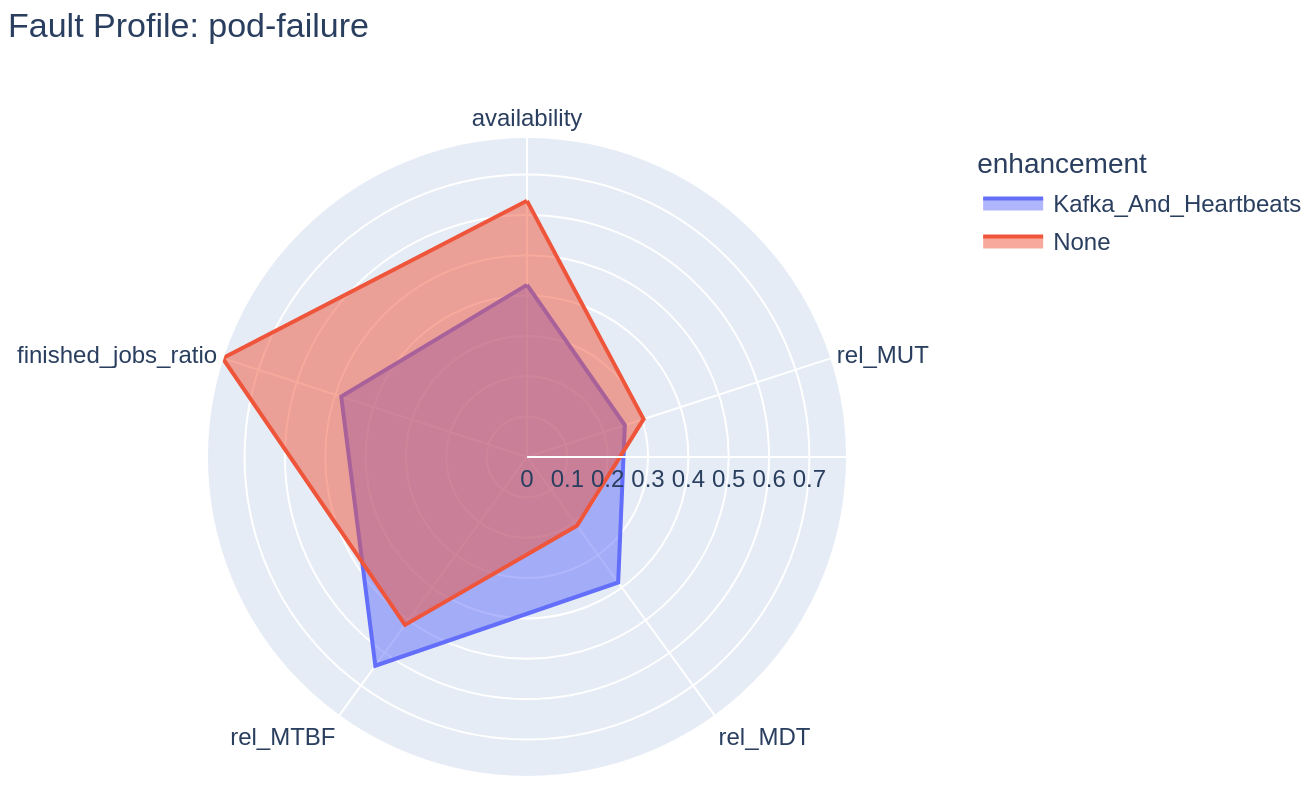
\includegraphics[width=140mm, keepaspectratio]{figures/kafka_and_hb_with_base_pod-failure.png}
	\caption{Combined enhancements - pod-failure fault profile}
	\label{fig:combined-results-pod-failure}
\end{figure}

\begin{figure}[h]
	\centering
	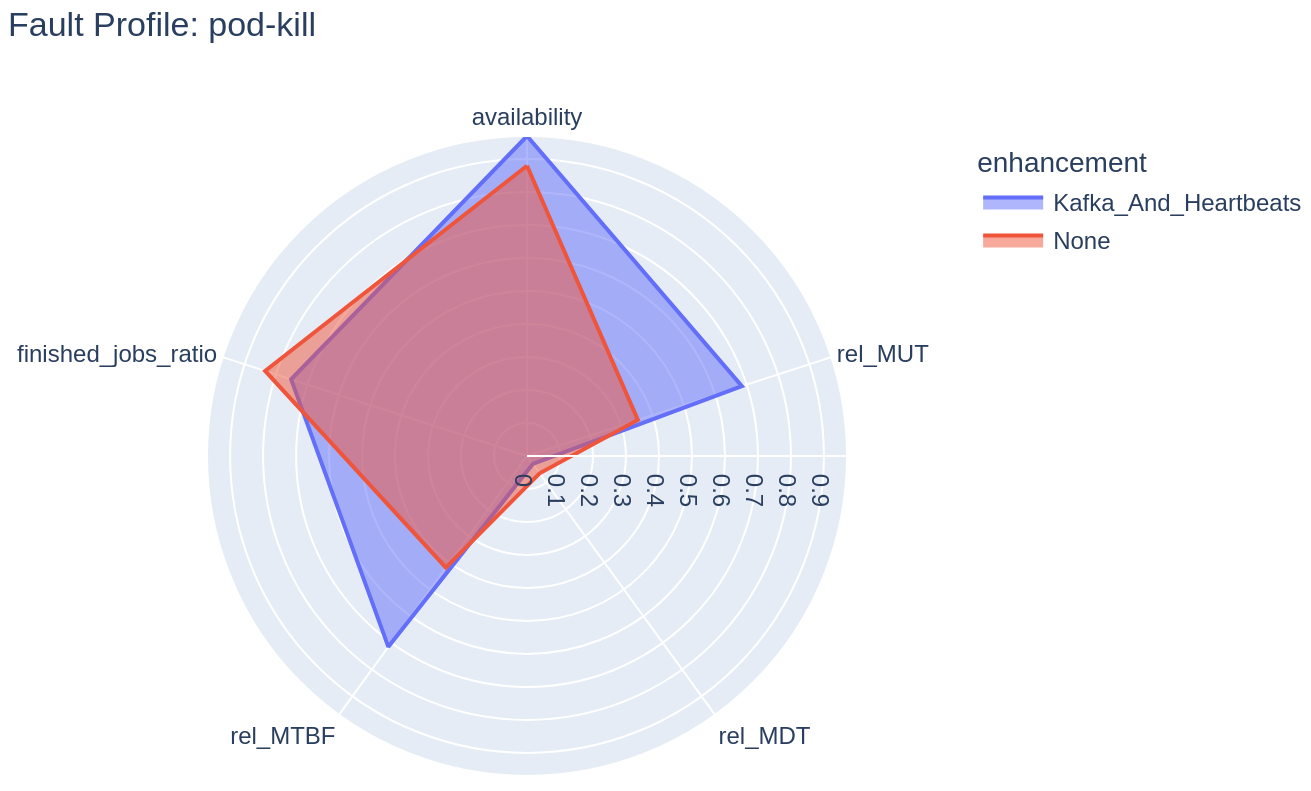
\includegraphics[width=140mm, keepaspectratio]{figures/kafka_and_hb_with_base_pod-kill.png}
	\caption{Combined enhancements - pod-kill fault profile}
	\label{fig:combined-results-pod-kill}
\end{figure}

